\begin{figure}[hbt]
  \centering
  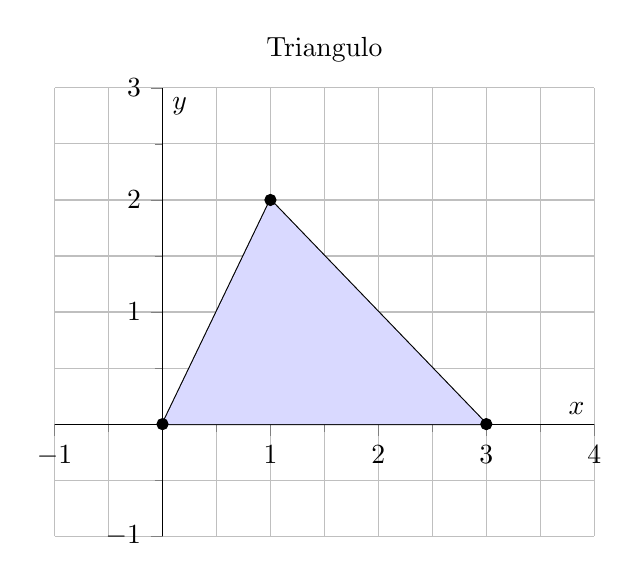
\begin{tikzpicture}
    \begin{axis}[
      xmin=-1, xmax=4,
      ymin=-1, ymax=3,
      axis x line=middle,
      axis y line=middle,
      axis line style={-},
      tick align=outside,
      grid=both,
      minor tick num=1,
      xlabel={$x$},
      ylabel={$y$},
      title={Triangulo}
    ]
      % Triângulo (fechando o caminho voltando ao primeiro ponto)
      \addplot[
        thick
      ] coordinates {
        (0,0)
        (3,0)
        (1,2)
        (0,0)
      };

      % Preenchimento opcional
      \addplot[
        fill=blue!15,
        draw=none
      ] coordinates {
        (0,0)
        (3,0)
        (1,2)
        (0,0)
      };

      % Pontos marcados
      \addplot[only marks, mark=*] coordinates {
        (0,0)
        (3,0)
        (1,2)
      };

    \end{axis}
  \end{tikzpicture}
  \caption{Ciclo Termodinâmico}
\end{figure}

%--------------------------------------------------
%somente por coordenadas
%--------------------------------------------------
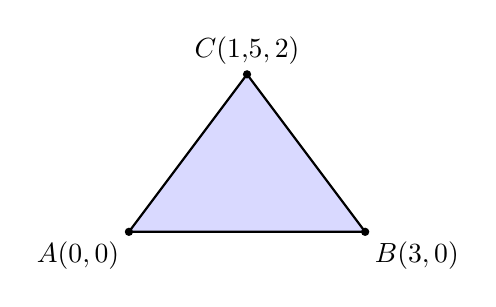
\begin{tikzpicture}
  % vértices
  \coordinate (A) at (0,0);
  \coordinate (B) at (3,0);
  \coordinate (C) at (1.5,2);

  % triângulo preenchido
  \fill[blue!15] (A) -- (B) -- (C) -- cycle;

  % contorno
  \draw[thick] (A) -- (B) -- (C) -- cycle;

  % marcar vértices
  \fill (A) circle (1.5pt) node[below left] {$A(0,0)$};
  \fill (B) circle (1.5pt) node[below right] {$B(3,0)$};
  \fill (C) circle (1.5pt) node[above] {$C(1{,}5,2)$};
\end{tikzpicture}

\begin{figure}[hbt]
  \centering
  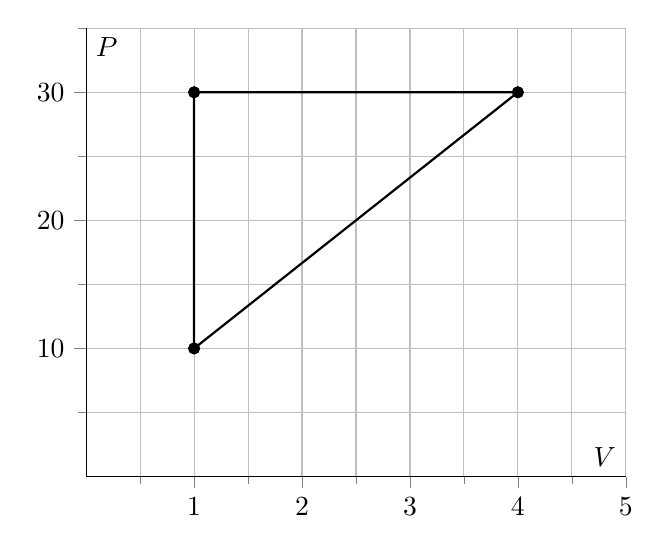
\begin{tikzpicture}
    \begin{axis}[
      xmin=0, xmax=5,
      ymin=0, ymax=35,
      axis x line=middle,
      axis y line=middle,
      axis line style={-},
      tick align=outside,
      grid=both,
      minor tick num=1,
      xlabel={$V$},
      ylabel={$P$},
      %title={Triângulo com vértices $(0,0)$, $(3,0)$ e $(1,2)$}
    ]
      % Triângulo (fechando o caminho voltando ao primeiro ponto)
      \addplot[
        thick
      ] coordinates {
        (1,10)
        (1,30)
        (4,30)
        (1,10)
      };

      % Preenchimento opcional
      % \addplot[
      %   fill=blue!15,
      %   draw=none
      % ] coordinates {
      %   (0,0)
      %   (3,0)
      %   (1,2)
      %   (0,0)
      % };

      % Pontos marcados
      \addplot[only marks, mark=*] coordinates {
        (1,10)
        (1,30)
        (4,30)
      };

    \end{axis}
  \end{tikzpicture}
  \caption{Triângulo definido pelas coordenadas dos vértices.}

  
\end{figure}